\documentclass[tikz]{standalone}
\usepackage{amsfonts}

% \usepackage{newtxtext,newtxmath}

%!TEX root = main.tex

% mytikzset
\usepackage{tikz}
\usetikzlibrary{positioning,arrows,shapes,patterns}
\usetikzlibrary{decorations.pathmorphing}
\usetikzlibrary{decorations.markings}
\usetikzlibrary{decorations.pathreplacing}
\usetikzlibrary{calc}
\usetikzlibrary{patterns}
\usetikzlibrary{decorations.markings}
\usetikzlibrary{petri}

\tikzset{
  vector/.style={thick,double,draw=black, postaction={decorate},
    decoration={markings,mark=at position .6 with {\arrow[black,scale=0.4]{triangle 45}}}},
  axial/.style={thick,double,densely dashed,draw=black, postaction={decorate},
    decoration={markings,mark=at position .6 with {\arrow[black,scale=0.4]{triangle 45}}}},
  gluon/.style={decorate, draw=black,
    decoration={coil,aspect=0.3,segment length=5pt,amplitude=3pt}},
  pseudo/.style={thick, dashed, draw=black, postaction={decorate},
    decoration={markings,mark=at position .6 with {\arrow[red,scale=0.5]{triangle 45}}}},
  scalar/.style={thick,draw=black, postaction={decorate},
    decoration={markings,mark=at position .6 with {\arrow[black,scale=0.5]{triangle 45}}}},
  cut/.style={draw=black, decorate, decoration={snake, segment length=1mm, amplitude=0.2mm}}
}


\newcommand{\Po}{\mathbb{P}}
\begin{document}
\nopagecolor
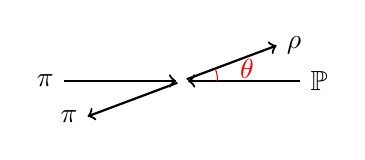
\begin{tikzpicture}[x=1.5cm,y=1.5cm]

\draw[<-, thick] (-0.05, 0)     --   (-1,0)    node[ left] {$\pi$ };
\draw[<-, thick] ( 0.05, 0)     --   ( 1,0)    node[right] {$\Po$ };
\draw[->, thick] ( 0.04, 0.015) -- ( 0.8, 0.3) node[right] {$\rho$};
\draw[->, thick] (-0.04,-0.015) -- (-0.8,-0.3) node[left] {$\pi$};

\draw[red] (0.3,0) arc (0:20:0.3) node[xshift=4mm] {\color{red} $\theta$};

\end{tikzpicture}
\end{document}
